%% How well it works

%% Discussion

%% Figures

\section{Results}
\subsubsection{Compute Performance}
Figure 10 illustrates the performance difference between DSPLIB provided FFT implementations vs the baseline fft.c. DSPLIB provides two separate implementations of FFT, the one in yellow is a decimation in time implementation for radix-2, whereas the one in blue is a mixed radix implementation. Points in read are from the baseline fft.c. The performance gap between the the baseline and optimized versions varies between 5x to 7x. I should be noted that although it was expected that FFT radix-2 perform better than mixed-radix, mix-radix consumes more memory than radix-2, and such benefits where in-place (radix-2) implementation suffers. Another thing to note is the slope of the two groups, which indicates the effect of bin-size on execution time. Since the number of executions are constant overall, this slope is indicative of cache-misses in the baseline code, which are minimal in the DSPLIB optimized versions.
\begin{figure}[h!]
  \caption{FFT Benchmark - DSPLIB vs Rulph's CS31 fft.c}
  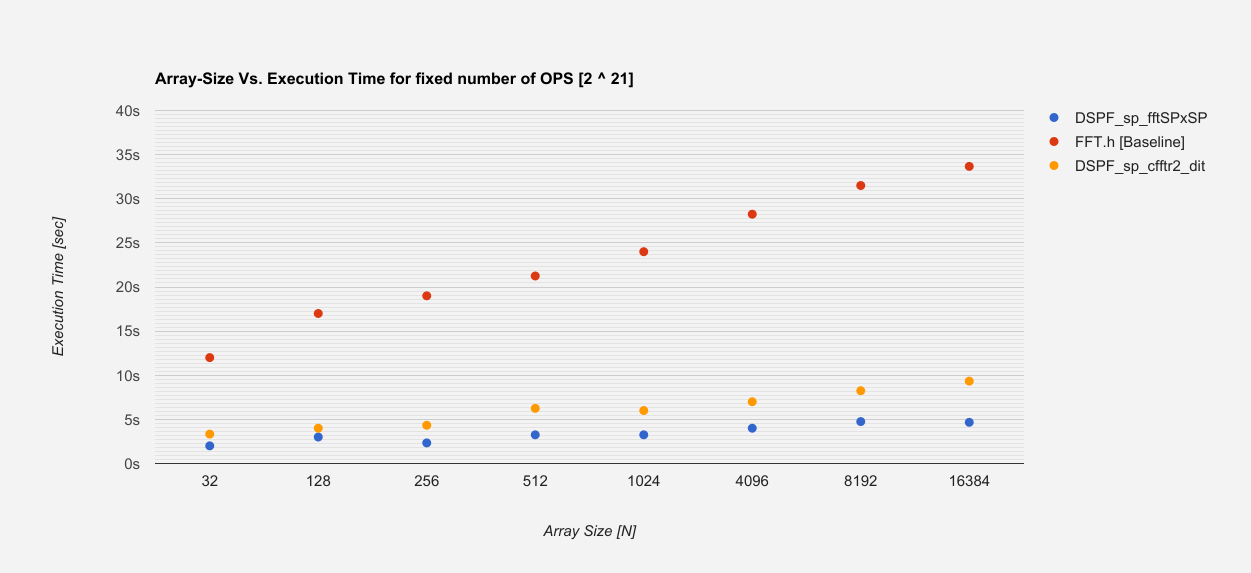
\includegraphics[width=0.5\textwidth]{images/fft.png}
\end{figure}\\

Figure 11 illustrates a performance evaluation between TI provided MATHLIB and TI compiler provided math.h. The x-axis represents number of clock cycles elapsed, and therefore faster code would be lesser. Comparisons are made for both single and double precision functions, and an oblivious improvement of nearly 2x is seen when using floats instead of doubles. It can also be seen that the MATHLIB implementations are another 2x faster, whereas vectorized implementations of all functions are nearly 15x to 22x faster. This is due to the pipeline and caching optimizations performed by MATHLIB, sources for which are available on this project's GitHub repo and on TI's website. 
\begin{figure}[h!]
  \caption{Math Benchmarks - MATHLIB vs math.h}
  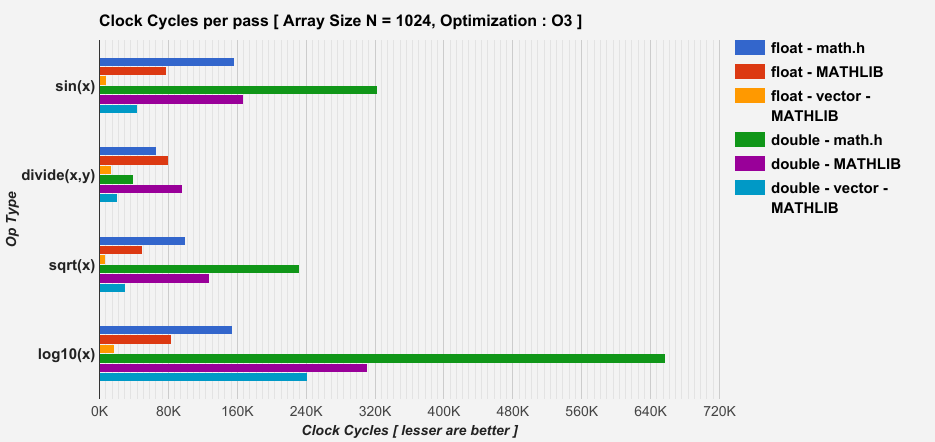
\includegraphics[width=0.5\textwidth]{images/math.png}
\end{figure}



%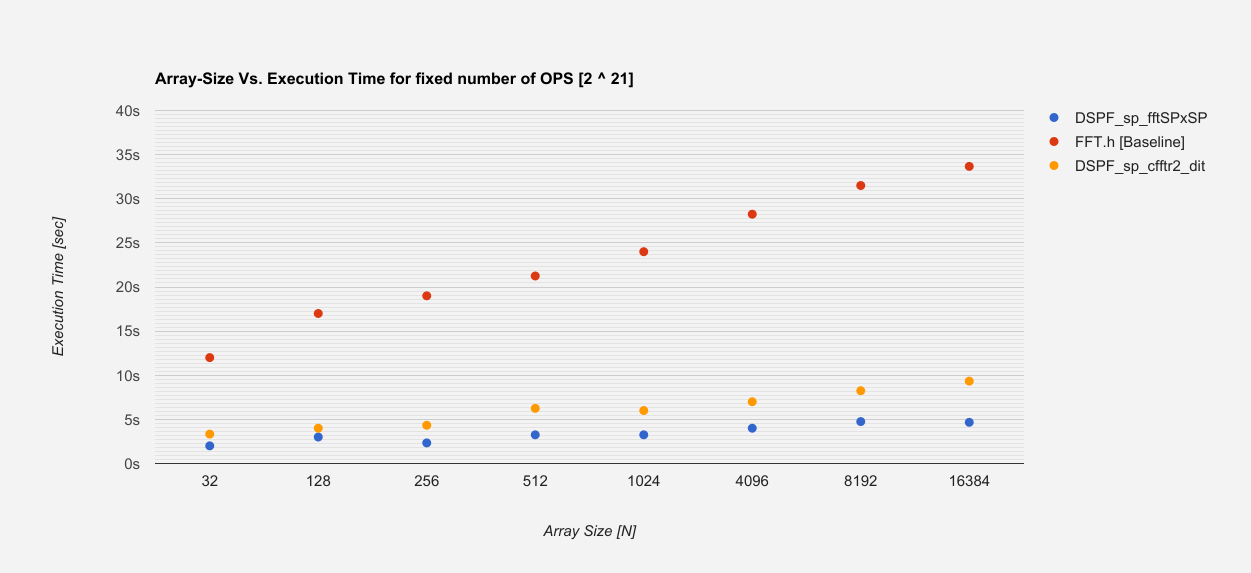
\includegraphics{images/fft.png}

\subsubsection{Communication Protocols}
All three protocols [I\textsuperscript{2}C, UART, GPIO] have been implemented and are known to be working well. All source code is available on GitHub, along with steps to reproduce the exact setup used in this project.\\

\subsubsection{Deep Neural Network}
Next, we test the efficacy of this system on a test data-set, and compare those results with two different instances of a RandomForest Classifier, one with 10 trees and another with 5000 trees. The training/test split (2149sec/114sec) is \emph{identical} for all three classifiers. The table below illustrates the results. 

\begin{center}
 \begin{tabular}{||c c c c||} 
 \hline
 Metrics & \textbf{DNN} & RForest (n=10) & RForest (n=5000) \\ [0.5ex] 
 \hline\hline
 Accuracy & 0.912 & 0.746 & 0.763 \\ 
 \hline
 Precision & 0.915 & 0.764 & 0.777 \\
 \hline
 Recall & 0.911 & 0.749 & 0.767 \\
 \hline
 \textbf{F-Measure} & \textbf{0.912} & 0.747 & 0.762 \\
 \hline
\end{tabular}
\end{center}

Over just a two second window-frame, the neural network was able to distinguish between stationary [sitting, standing, laying down] and walking positions with around $91.2\%$ accuracy, while RandomForest(n=10) could manage a meagre $74.7\%$. Even when given the opportunity to over-fit and memorize the entire training set (n=5000), the RandomForest classifier did not improve. This confirms two distinct hypotheses: first, the test-data is distinct enough from training that memorizing does not seem to improve the prediction score; and second, the neural network is indeed learning, not just memorizing the data-set either. \\

This test succinctly highlights one of the biggest strengths of neural networks, i.e. the ability to extract features implicitly from within a raw-signal, without the need for additional prepossessing and feature-extraction. 
